\documentclass[a4paper,12pt]{article}
\usepackage[utf8]{inputenc}
\usepackage[brazilian]{babel}

\usepackage{mathptmx}               %Times New Roman
\usepackage{newtxtext,newtxmath} 

\usepackage{setspace}
\setstretch{1}      % Espacio entre lineas

\usepackage{vmargin}
\setpapersize{A4}
\setmargins{3cm}	% margen izquierdo
{1.5cm}            	% margen superior
{15cm}          	% anchura del texto
{23.5cm}          	% altura del texto
{10pt}             	% altura de los encabezados
{1cm}              	% espacio entre el texto y los encabezados
{0pt}              	% altura del pie de página
{1.5cm}             % espacio entre el texto y el pie de página

\usepackage{cite}

\usepackage{flushend}
\usepackage{amsmath}
\usepackage{textcomp}

\usepackage{multirow}

\usepackage[usenames]{color}
\usepackage[hidelinks]{hyperref} 

\usepackage{enumitem,kantlipsum}

\usepackage{graphicx} % figuras
\usepackage[export]{adjustbox}
\usepackage[labelfont=bf]{caption} %Negrita al label de la figura
\usepackage[font=it]{caption} %Italica descripcion de la figura 

\usepackage{fancyhdr,lipsum} %Encabezados
\pagestyle{fancy}
\setlength{\headheight}{52pt}

\fancypagestyle{plain}{
\fancyhead[L]{}
\fancyhead[R]{CAP-241-4 - Computação Aplicada}
\setlength{\headheight}{15pt}
\renewcommand{\headrulewidth}{0.5pt}}

\usepackage{subcaption}

\usepackage{breqn}

\usepackage{verbatim} 

% xmark
\usepackage{amssymb}% http://ctan.org/pkg/amssymb
\usepackage{pifont}% http://ctan.org/pkg/pifont
\newcommand{\cmark}{\ding{51}}%
\newcommand{\xmark}{\ding{55}}%

\begin{document}

\begin{figure}
 \begin{center}
  
\includegraphics[width=1\linewidth]{fig/logoinpe.png}
 \end{center}
\end{figure}

\setlength{\textfloatsep}{0pt}

\title{Modelando Epidemias Usando Autômatos Celulares}
    
\author{Cesar Arturo Sánchez Pena \\ Felipe Menino Carlos}
\date{}

\maketitle

\section{Introdução}

Modelos são formas de representação simplificadas de sistemas da natureza e seus comportamentos, utilizados para que os pontos mais importantes e relevantes sejam vistos e compreendidos (KIER 2005\cite{Kier2005}). Diversos estudos usam de modelos para o entendimento do comportamento geral de sistemas da natureza com os mais diferentes objetivos e necessidades. Alguns exemplos podem ser encontrados em Cairo \textit{et al} 2019 \cite{Cairo2019}, que utiliza de modelos estatísticos para a modelagem de concentração de chl-\textit{a} através de dados de Sensoriamento Remoto; Outro exemplo está em ZORZENON \textit{et al} \cite{ZorzenonDosSantos2001}, que estuda a evolução do Vírus da Imunodeficiência Humana (HIV). % \vspace{12pt}

O processo de modelagem pode ser feito através da utilização de diversas técnicas (KIER 2005\cite{Kier2005}). Atualmente, dentre as técnicas utilizadas está o Autômato Celular (AC), que através de um conjunto de regras simples, permitem a modelagem de sistemas e comportamentos complexos (MELOTTI 2009\cite{Melotti2009}). % \vspace{12pt}

Dentro do contexto da modelagem epidemiológica, os ACs tem sido amplamente utilizados por considerar características que as abordagens clássicas (baseadas em equações diferenciais), podem não representar. De acordo com White 2007 \cite{White2007} e Sirakou 2000\cite{Sirakoulis2000}, dentre essas características estão: $(i)$ O processo de contato individual; $(ii)$ comportamentos individuais; $(iii)$ aspectos espaciais da propagação; e $(iv)$ efeito dos padrões de mistura dos indivíduos. % \vspace{12pt}

Com isto, o presente trabalho tem por objetivo implementar, analisar e comparar o modelo de AC determinístico, criado para a simulação geral de epidemias, considerando características de transmissão e controle da doença, proposto por White 2007\cite{White2007}, Além disso, é apresentado uma implementação do modelo em que um mapa dos estados do Brasil é usado como espaço celular.

\section{Modelo de Propagação Epidêmica}

\par ACs são modelos matemáticos que tornam possível a representação de sistemas e fenômenos dinâmicos (MELOTTI 2009 \cite{Melotti2009} e CASTRO 2008 \cite{Castro2008}), tornando esses ferramentas úteis para a modelagem de diferentes tipos de comportamento, sendo empregados nos mais variados contextos (CASTRO 2008\cite{Castro2008}). Liu 2008 \cite{Liu2008} apresenta que os ACs possuem cinco elementos fundamentais em sua composição, sendo eles: $(i)$ Célula, o elemento base do AC, disposto em um \textit{grid} \textit{n}-dimensional, nomeado de Espaço Celular; $(ii)$ Estado, que é atribuído a uma célula; $(iii)$ Vizinhança, utilizada para a determinação de interação entre as células. Para estas, os tipos mais utilizados são o de \texttt{Von Neumann} e \texttt{Moore} (ALEXANDER 2008 \cite{alexanderschatten2008}); $(iv)$ Regra de transição, que utilizando da vizinhança determina o estado atual do autômato; e $(v)$ Tempo, que é utilizado para aplicar, a atualização dos estados do autômato através da aplicação das Regras de Transição. 

Com base em tais características, White 2007\cite{White2007} propuseram um modelo de AC para a simulação de epidemias. No modelo proposto é considerado que cada célula representa uma cidade, com uma determinada população. Entre cada célula é considerado a locomoção de indivíduos e meios de transporte para tal. Por fim é tido também que não há nascimentos ou mortes na população, o que faz a população geral permanecer a mesma.

\subsection{População}
Como descrito por White 2007\cite{White2007}, para a representação da população dentro do AC é assumido que, o terreno onde a epidemia está ocorrendo é representado pelo espaço celular bidimensional $MxN$, com células de geometria quadrada e áreas idênticas. Dentro de cada uma das células $(i,j)$ é tido que existe uma população de indivíduos $N_{ij}$, com distribuição não-homogênea, isto é, quantidades de indivíduos diferentes na população das células. O modelo apresentado é do tipo Suscetíveis-Infectados-Recuperados (SIR), assim, cada indivíduo dentro das populações das células podem ser dos tipos suscetíveis $S_{ij}^t \in [0, 1]$, infectados $I_{ij}^t \in [0, 1]$ e recuperados $R_{ij}^t \in [0, 1]$, de modo que estes juntos devem respeitar a regra $S_{ij}^t + I_{ij}^t + R_{ij}^t = 1$. Neste modelo, só são infectados os suscetíveis, e após um tempo infectado é possível passar para o estado recuperado, sendo que, neste estado, não há mais mudança para tal indivíduo. A maneira com que a infecção ocorre é descrita através da relação entre os indivíduos infectados da mesma célula ou com células vizinhas. 

\subsection{Função de transição}

A função de transição faz a determinação do estado de cada célula através de três equações, uma para cada tipo de indivíduo da população. As equações que definem o sistema são:

\begin{equation} 
I_{ij}^t=\left(1\:-\:\varepsilon \right)\cdot I_{ij}^{t\:-\:1}+v\:\cdot S_{ij}^{t\:-\:1}\cdot I_{ij}^{t\:-\:1}+S_{ij}^{t\:-\:1}\cdot \:\displaystyle \:\sum _{\left(\alpha ,\beta \right)\in V^{\ast }}^{ }\left(\frac{N_{i+\alpha ,\:j\:+\:\beta }}{N_{ij}}\cdot \mu _{\alpha \beta }^{\left(i,\:j\right)}\cdot I_{i+\alpha \:,\:j+\beta \:}^{t\:-\:1}\:\right)
\label{eq1}
\end{equation}

\begin{equation}
S_{ij}^t=S_{ij}^{t\:-\:1}-v\cdot S_{ij}^{t\:-\:1}\cdot I_{ij}^{t\:-\:1}-S_{ij}^{t\:-\:1}\cdot \:\displaystyle \:\sum _{\left(\alpha ,\beta \right)\in V^{\ast }}^{ }\left(\frac{N_{i+\alpha ,\:j\:+\:\beta }}{N_{ij}}\cdot \mu _{\alpha \beta }^{\left(i,\:j\right)}\cdot I_{i+\alpha \:,\:j+\beta \:}^{t\:-\:1}\:\right)
\label{eq2}
\end{equation}

\begin{equation} 
R_{ij}^t=R_{ij}^{t\:-\:1}+\varepsilon \cdot I_{ij}^{t\:-\:1}
\label{eq3}
\end{equation}

A variável $V^\star$ representa todos os vizinhos de uma célula e o parâmetro $\mu_{\alpha \beta}^{\left(i,\:j\right)}$ é definido como:

\begin{equation}
\mu_{\alpha \beta}^{\left(i,\:j\right)} = c_{\alpha\beta}^{\left(i,\:j\right)} m_{\alpha \beta}^{\left(i,\:j\right)}v
\end{equation}

Onde $c_{\alpha \beta}^{\left(i,\:j\right)} \in [0, 1]$ e $ m_{\alpha \beta}^{\left(i,\:j\right)} \in [0, 1]$ representam o fator de conexão entre as células e o fator de movimento entre a célula e seus vizinhos $(i + \alpha, j + \beta)$, respectivamente. O fator $v \in [0, 1]$ representa a virulência da epidemia e $\varepsilon \in [0, 1]$ indica o fator de recuperação dos indivíduos infectados.

Para a Equação \ref{eq1}, na primeira soma, é tido que os infectados no tempo $t$ serão representados pela porção de indivíduos do tempo anterior ($t-1$) que não foram curados. O segundo termo mostra a porção dos indivíduos saudáveis que foram infectados pelo contato direito, aqui é levado em conta o fator de virulência, este termo é proporcional na agressividade do vírus. O último termo apresenta os que foram infectados por contato com vizinhos infectados. Na Equação \ref{eq2} tem-se comportamento análogo ao apresentado, porém considerando os suscetíveis. Finalmente a Equação \ref{eq3}, apresenta a proporção de indivíduos recuperados para o tempo $t$.

\subsection{Conexão e Movimento}

Os fatores de \texttt{Conexão} e \texttt{Movimento}, podem ser interpretados respectivamente como,a quantidade de serviços que o indivíduo tem disponível para a movimentação entre as células e a probabilidade de cada indivíduo em utilizar tais serviços. Durante a descrição do fator de Conexão White 2007 \cite{White2007} faz uma relação com meios de transporte como avião, ônibus e carro entre cada célula e determina um fator que represente cada um desses meios de transporte. Essa relação de fatores é apresentada na Tabela \ref{tab:movimentacao}. 

\begin{table}[ht]
 \caption{Discretização do transporte. Adaptado de WHITE 2007\cite{White2007}.}
 \centering
 \begin{tabular}{c|c|c|c|c}
  Conectividade & Fator & Avião & Ônibus & Carro \\
  \hline
  \multirow{4}{*}{$c_{\alpha \beta}^{\left(i,\:j\right)}$} & 1 & \cmark & \cmark & \cmark \\
  & 0.6 & \xmark & \cmark & \cmark \\
  & 0.3 & \xmark & \xmark & \cmark \\
  & 0   & \xmark & \xmark & \xmark \\
\end{tabular}
\label{tab:movimentacao}
\end{table}

\subsection{Vacinação}

Como forma de adicionar um fator de controle para a epidemia, o AC considerado neste trabalho, utiliza um fator para a representação do processo de vacinação que é aplicado na população de cada célula. As equações para este caso tem comportamento análogo ao já apresentado anteriormente, com a diferença de que, nessas há o fator $\omega \in [0, 1]$, que representa a proporção de indivíduos vacinados em cada célula. Tais mudanças são apresentadas nas Equações \ref{eq:vacineS} e \ref{eq:vacineR}, não havendo mudanças para o comportamento dos infectados.

\begin{equation} 
S_{ij}^t=S_{ij}^{t\:-\:1}-\omega \cdot S_{ij}^{t\:-\:1}-v\cdot \:S_{ij}^{t\:-\:1}\cdot \:I_{ij}^{t\:-\:1}-S_{ij}^{t\:-\:1}\cdot \:\displaystyle \:\sum _{\left(\alpha ,\beta \right)\in V^{\ast }}^{ }\left(\frac{N_{i+\alpha ,\:j\:+\:\beta }}{N_{ij}}\cdot \mu _{\alpha \beta }^{\left(i,\:j\right)}\cdot I_{i+\alpha \:,\:j+\beta \:}^{t\:-\:1}\:\right)
\label{eq:vacineS}
\end{equation}

\begin{equation} 
R_{ij}^t=R_{ij}^{t\:-\:1}+\varepsilon \:\cdot \:I_{ij}^{t\:-\:1}+\omega \cdot S_{ij}^{t\:-1}
\label{eq:vacineR}
\end{equation}

\section{Resultados}

Esta Seção é dividida em duas partes, sendo que, a primeira apresenta a implementação base do modelo junto aos testes propostos em White 2007\cite{White2007} e a segunda parte mostra um exemplo de espacialização do modelo. As implementações\footnote{O código desenvolvido e animações criadas está disponível no GitHub (\href{https://github.com/M3nin0/epidemic-model}{https://bit.ly/2KfYnf7})} do modelo base foram feitas utilizando a plataforma de modelagem TerraME (CARNEIRO 2013 \cite{CARNEIRO2013104}) e o processo de espacialização foi feito em Python.

\subsection{Simulações base}

Como forma de ilustrar o comportamento do modelo com diferentes conjuntos de parâmetros, esta Seção faz diferentes testes variando os parâmetros de simulação do modelo. Para todos os testes é utilizado um espaço celular de 50x50, sendo que, o ponto inicial da epidemia em todos os casos ocorre a partir da célula $(25,25)$ e todas as células tem população $N_{ij}$ igual a 100. Nos testes realizados são considerados as vizinhanças de Moore e Von Neumann. % \\

O primeiro caso de testes assume o mesmo conjunto de parâmetros utilizados por White 2007\cite{White2007}, onde para a célula de início da epidemia, tem-se uma população dividida em 70\% de suscetíveis e 30\% de infectados, e que os valores dos parâmetros utilizados no modelo são, $v$ = 0.6, $\varepsilon$ = 0.4 e  $ m_{\alpha \beta}^{\left(i,\:j\right)}$ = 0.5. É considerado também que o fator de conexão $c_{\alpha \beta}^{\left(i,\:j\right)}$ é 1, para todas as células. 

A Figura \ref{figure:exp1moore} apresenta os resultados da simulação utilizando a vizinhança de Moore e na Figura \ref{figure:exp1vonneumann} são apresentados os resultados da simulação com a vizinhança de Von Neumann. As cores das Figuras representam a quantidade de infectados nas células, indo do branco ao vermelho, com tons de cinza como intermediários. Assim, o branco representa que não há infectados e o vermelho representa que toda a população da célula foi infectada. 

\newpage 

\begin{figure}[!ht]
\captionsetup[subfigure]{labelformat=empty}
\centering
\subfloat[\textit{t} = 1]{{\includegraphics[height=2.5cm,width=2.5cm, frame]{fig/experimentos_base/images_parametros_padrao_teste_modelo_moore/epidemicmodel_t1.png}}}
\qquad
\subfloat[\textit{t} = 5]{{\includegraphics[height=2.5cm,width=2.5cm, frame]{fig/experimentos_base/images_parametros_padrao_teste_modelo_moore/epidemicmodel_t5.png}}}
\qquad
\subfloat[\textit{t} = 15]{{
\includegraphics[height=2.5cm,width=2.5cm, frame]{fig/experimentos_base/images_parametros_padrao_teste_modelo_moore/epidemicmodel_t15.png}}}
\qquad
\subfloat[\textit{t} = 20]{{
\includegraphics[height=2.5cm,width=2.5cm, frame]{fig/experimentos_base/images_parametros_padrao_teste_modelo_moore/epidemicmodel_t20.png}}}
\qquad
\subfloat[\textit{t} = 25]{{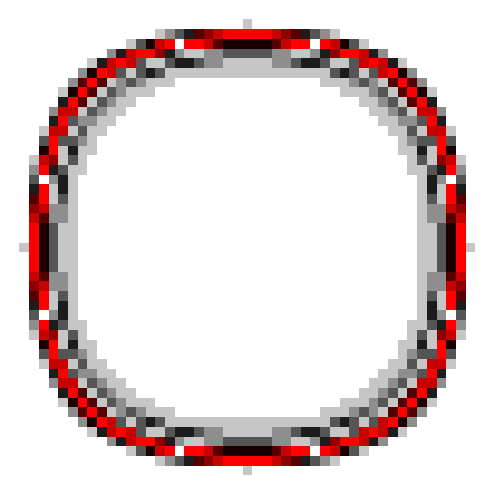
\includegraphics[height=2.5cm,width=2.5cm, frame]{fig/experimentos_base/images_parametros_padrao_teste_modelo_moore/epidemicmodel_t25.png}}}
\qquad
\subfloat[\textit{t} = 30]{{
\includegraphics[height=2.5cm,width=2.5cm, frame]{fig/experimentos_base/images_parametros_padrao_teste_modelo_moore/epidemicmodel_t30.png}}}
\qquad
\subfloat[\textit{t} = 35]{{
\includegraphics[height=2.5cm,width=2.5cm, frame]{fig/experimentos_base/images_parametros_padrao_teste_modelo_moore/epidemicmodel_t35.png}}}
\qquad
\subfloat[\textit{t} = 40]{{
\includegraphics[height=2.5cm,width=2.5cm, frame]{fig/experimentos_base/images_parametros_padrao_teste_modelo_moore/epidemicmodel_t40.png}}}
\caption{Simulação com população constante e vizinhança de Moore}
\label{figure:exp1moore}
\end{figure}

\begin{figure}[!ht]
\captionsetup[subfigure]{labelformat=empty}
\centering
\subfloat[\textit{t} = 1]{{\includegraphics[height=2.5cm,width=2.5cm, frame]{fig/experimentos_base/images_parametros_padrao_teste_modelo_vonneumann/epidemicmodel_t1.png}}}
\qquad
\subfloat[\textit{t} = 5]{{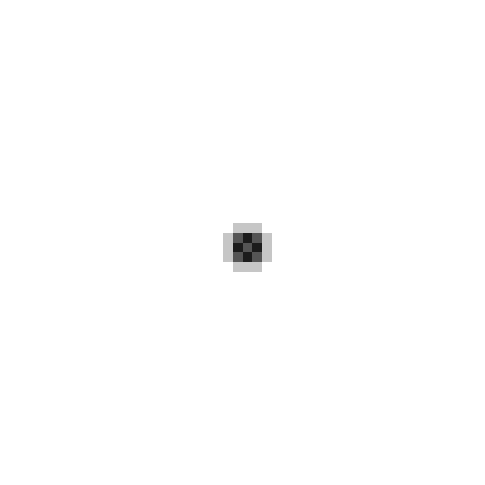
\includegraphics[height=2.5cm,width=2.5cm, frame]{fig/experimentos_base/images_parametros_padrao_teste_modelo_vonneumann/epidemicmodel_t5.png}}}
\qquad
\subfloat[\textit{t} = 15]{{
\includegraphics[height=2.5cm,width=2.5cm, frame]{fig/experimentos_base/images_parametros_padrao_teste_modelo_vonneumann/epidemicmodel_t15.png}}}
\qquad
\subfloat[\textit{t} = 20]{{
\includegraphics[height=2.5cm,width=2.5cm, frame]{fig/experimentos_base/images_parametros_padrao_teste_modelo_vonneumann/epidemicmodel_t20.png}}}
\qquad
\subfloat[\textit{t} = 25]{{
\includegraphics[height=2.5cm,width=2.5cm, frame]{fig/experimentos_base/images_parametros_padrao_teste_modelo_vonneumann/epidemicmodel_t25.png}}}
\qquad
\subfloat[\textit{t} = 30]{{
\includegraphics[height=2.5cm,width=2.5cm, frame]{fig/experimentos_base/images_parametros_padrao_teste_modelo_vonneumann/epidemicmodel_t30.png}}}
\qquad
\subfloat[\textit{t} = 35]{{
\includegraphics[height=2.5cm,width=2.5cm, frame]{fig/experimentos_base/images_parametros_padrao_teste_modelo_vonneumann/epidemicmodel_t35.png}}}
\qquad
\subfloat[\textit{t} = 40]{{
\includegraphics[height=2.5cm,width=2.5cm, frame]{fig/experimentos_base/images_parametros_padrao_teste_modelo_vonneumann/epidemicmodel_t40.png}}}
\caption{Simulação com população constante e vizinhança de Von Neumann}
\label{figure:exp1vonneumann}
\end{figure}

Como é possível perceber nas Figuras apresentadas, as simulações utilizando as vizinhanças de Moore apresentam estágios bem maiores de infecção do que as simulações feitas utilizando as vizinhanças de Von Neumann, o que pode ser explicado pela quantidade de vizinhos que cada célula tem contato de uma única vez. Ao ter mais contato com outras células, a chance de contaminação é maior. Este comportamento pode ser melhor visualizado na Figura \ref{figure:exp1graph}, que apresenta a quantidade total de cada um dos tipos de população durante a simulação, frente aos diferentes tipos de vizinhanças.

\newpage

Partindo dos testes desta primeira simulação, percebe-se que é importante entender a maneira como o fator de conexão entre as células afeta a epidemia modelada, considerando isto, para a realização de uma nova simulação de teste é considerado o método de divisão do espaço celular apresentado por White 2007 \cite{White2007}, neste, o espaço celular é dividido em quatro quadrantes, sendo que para cada um desses quadrantes é atribuído um fator de conectividade.

\begin{figure}[!ht]
\centering
\subfloat[Moore]{{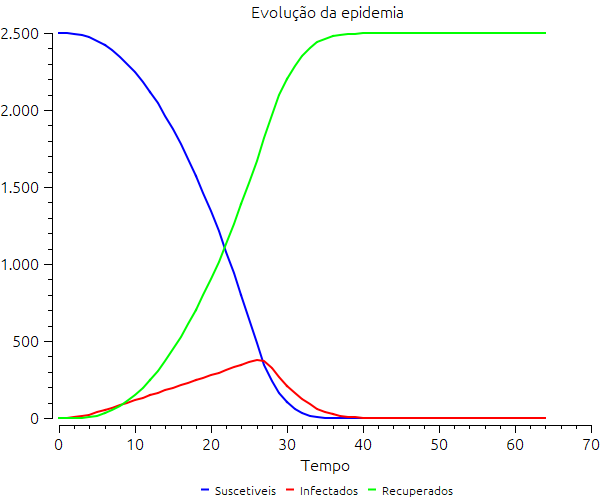
\includegraphics[height=5.5cm,width=5.5cm, frame]{fig/experimentos_base/images_parametros_padrao_teste_modelo_moore/epidemicmodel_finalchart.png}}}
\qquad
\subfloat[Von Neumann]{{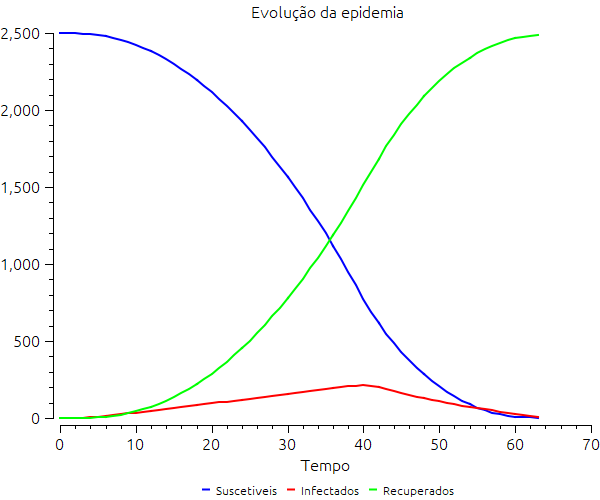
\includegraphics[height=5.5cm,width=5.5cm, frame]{fig/experimentos_base/images_parametros_padrao_teste_modelo_vonneumann/epidemicmodel_finalchart.png}}}
\caption{Simulação com diferentes formas de vizinhanças}
\label{figure:exp1graph}
\end{figure}

A distribuição das conectividades do espaço celular podem ser vistos na Figura \ref{figure:artificialCellSpace}, onde as tonalidades de cores representam o grau do fator de conexão, quanto mais escuro, maior o grau de conexão. Assim, as áreas $C_1$ e $C_2$ possuem os maiores fatores de conectividade, sendo respectivamente os valores 0.6 e 1. Já as áreas $C_3$ e $C_4$ possuem fatores de conectividade menor, sendo esses 0 e 0.3, respectivamente. 

\begin{figure}[!ht]
 \begin{center}
  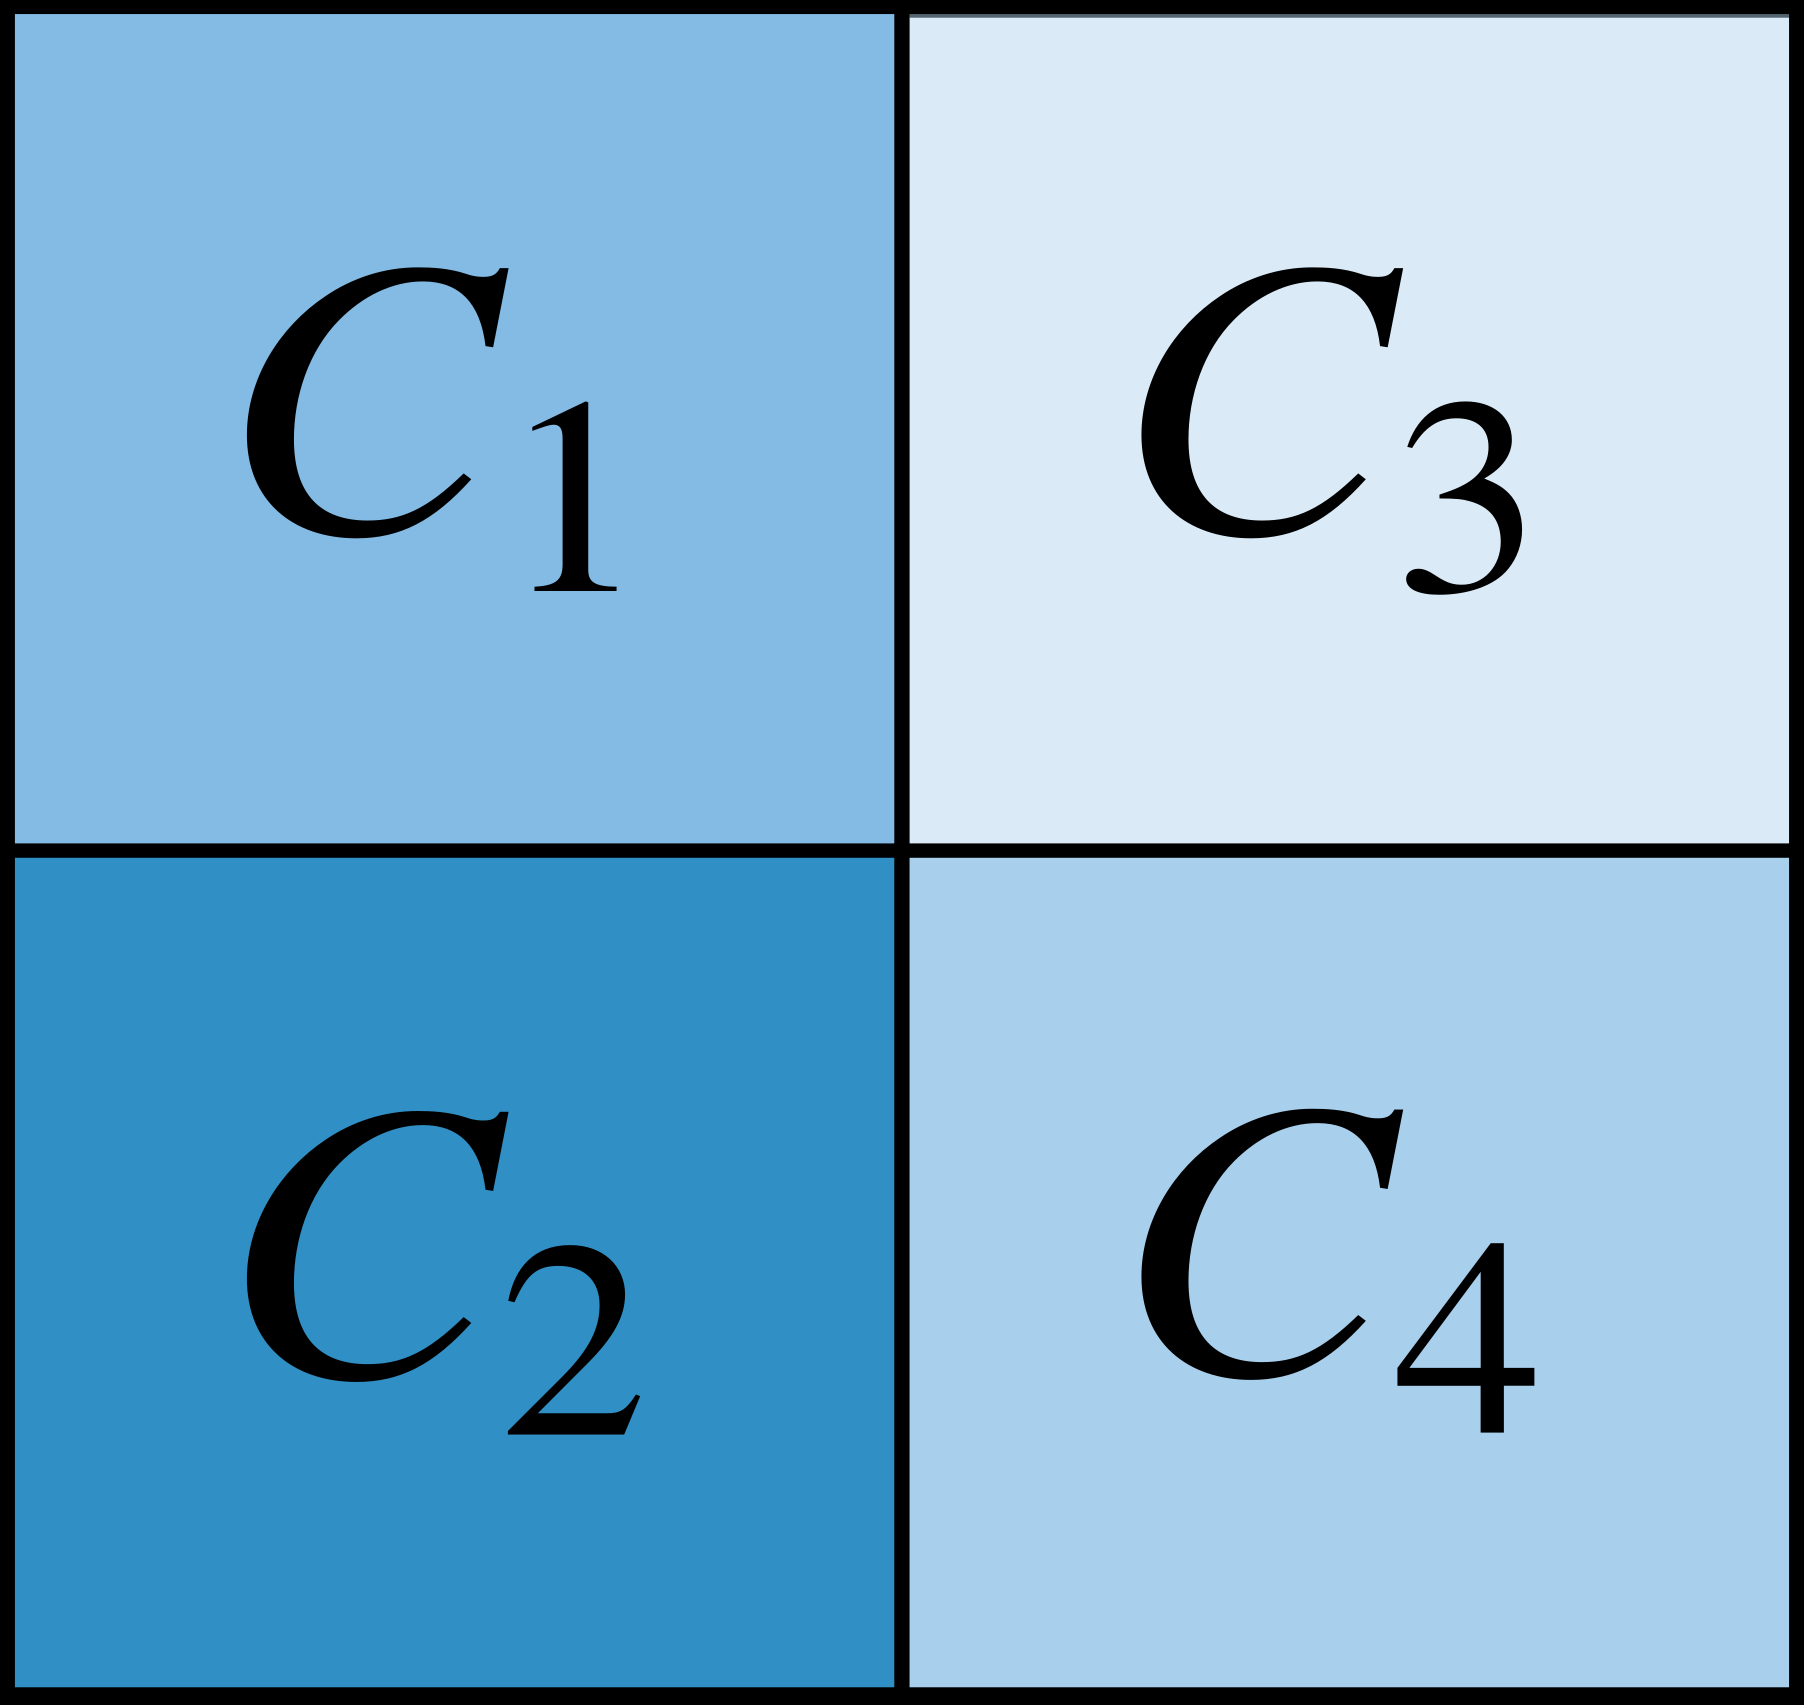
\includegraphics[width=0.35\linewidth]{fig/area_artificial.png}
 \end{center}
 \caption{Espaço celular com quadrantes diferentes de conectividade}
\label{figure:artificialCellSpace}
\end{figure}

Com isso, ao realizar as simulações, tanto para os testes de vizinhanças de Moore (Figura \ref{figure:exp2moore}) quanto de Von Neumann (Figura \ref{figure:exp2vonneumann}), é possível perceber que as áreas que representam $C_1$ e $C_2$, por dispor de maior conectividade, fizeram o vírus se espalhar mais rápido, enquanto que no quadrante $C_3$, por não possuir conexão com outras células, não teve nenhuma infecção e no $C_4$, seguindo a lógica, a transmissão foi muito baixa. 

\newpage
É importante citar também que, o mesmo comportamento do número de infectados apresentados na Figura \ref{figure:exp1graph} foi encontrado aqui, onde as simulações com Moore tiveram mais casos de células totalmente infectadas do que as simulações feitas com Von Neumann.

\begin{figure}[!ht]
\captionsetup[subfigure]{labelformat=empty}
\centering
\subfloat[\textit{t} = 1]{{\includegraphics[height=2.5cm,width=2.5cm, frame]{fig/experimentos_base/images_parametros_padrao_area_artificial_moore/epidemicmodel_t1.png}}}
\qquad
\subfloat[\textit{t} = 5]{{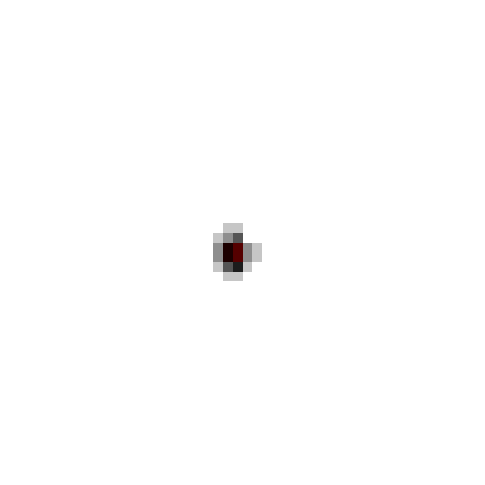
\includegraphics[height=2.5cm,width=2.5cm, frame]{fig/experimentos_base/images_parametros_padrao_area_artificial_moore/epidemicmodel_t5.png}}}
\qquad
\subfloat[\textit{t} = 10]{{
\includegraphics[height=2.5cm,width=2.5cm, frame]{fig/experimentos_base/images_parametros_padrao_area_artificial_moore/epidemicmodel_t10.png}}}
\qquad
\subfloat[\textit{t} = 15]{{
\includegraphics[height=2.5cm,width=2.5cm, frame]{fig/experimentos_base/images_parametros_padrao_area_artificial_moore/epidemicmodel_t15.png}}}
\qquad
\subfloat[\textit{t} = 25]{{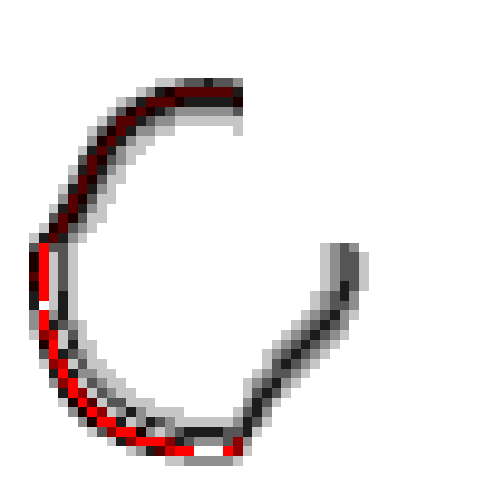
\includegraphics[height=2.5cm,width=2.5cm, frame]{fig/experimentos_base/images_parametros_padrao_area_artificial_moore/epidemicmodel_t25.png}}}
\qquad
\subfloat[\textit{t} = 35]{{
\includegraphics[height=2.5cm,width=2.5cm, frame]{fig/experimentos_base/images_parametros_padrao_area_artificial_moore/epidemicmodel_t35.png}}}
\qquad
\subfloat[\textit{t} = 50]{{
\includegraphics[height=2.5cm,width=2.5cm, frame]{fig/experimentos_base/images_parametros_padrao_area_artificial_moore/epidemicmodel_t50.png}}}
\qquad
\subfloat[\textit{t} = 60]{{
\includegraphics[height=2.5cm,width=2.5cm, frame]{fig/experimentos_base/images_parametros_padrao_area_artificial_moore/epidemicmodel_t65.png}}}
\caption{Simulação com população constante e vizinhança de Moore com conectividade por quadrante}
\label{figure:exp2moore}
\end{figure}

\begin{figure}[!ht]
\captionsetup[subfigure]{labelformat=empty}
\centering
\subfloat[\textit{t} = 1]{{\includegraphics[height=2.5cm,width=2.5cm, frame]{fig/experimentos_base/images_parametros_padrao_area_artificial_vonneumann/epidemicmodel_t1.png}}}
\qquad
\subfloat[\textit{t} = 5]{{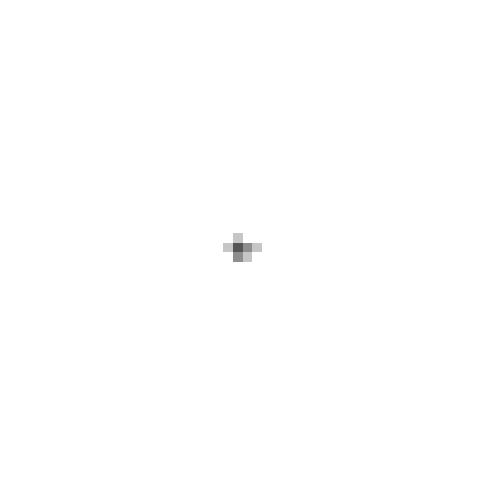
\includegraphics[height=2.5cm,width=2.5cm, frame]{fig/experimentos_base/images_parametros_padrao_area_artificial_vonneumann/epidemicmodel_t5.png}}}
\qquad
\subfloat[\textit{t} = 10]{{
\includegraphics[height=2.5cm,width=2.5cm, frame]{fig/experimentos_base/images_parametros_padrao_area_artificial_vonneumann/epidemicmodel_t10.png}}}
\qquad
\subfloat[\textit{t} = 15]{{
\includegraphics[height=2.5cm,width=2.5cm, frame]{fig/experimentos_base/images_parametros_padrao_area_artificial_vonneumann/epidemicmodel_t15.png}}}
\qquad
\subfloat[\textit{t} = 25]{{
\includegraphics[height=2.5cm,width=2.5cm, frame]{fig/experimentos_base/images_parametros_padrao_area_artificial_vonneumann/epidemicmodel_t25.png}}}
\qquad
\subfloat[\textit{t} = 35]{{
\includegraphics[height=2.5cm,width=2.5cm, frame]{fig/experimentos_base/images_parametros_padrao_area_artificial_vonneumann/epidemicmodel_t35.png}}}
\qquad
\subfloat[\textit{t} = 50]{{
\includegraphics[height=2.5cm,width=2.5cm, frame]{fig/experimentos_base/images_parametros_padrao_area_artificial_vonneumann/epidemicmodel_t50.png}}}
\qquad
\subfloat[\textit{t} = 60]{{
\includegraphics[height=2.5cm,width=2.5cm, frame]{fig/experimentos_base/images_parametros_padrao_area_artificial_vonneumann/epidemicmodel_t65.png}}}
\caption{Simulação com população constante e vizinhança de Von Neumann com conectividade por quadrante}
\label{figure:exp2vonneumann}
\end{figure}

Até este ponto, todas as simulações foram feitas com população constante, como já citado anteriormente, porém, o modelo analisado neste trabalho da margem para a variação da população, indicando que tal variação afeta diretamente no efeito da epidemia que está sendo gerado, desta forma, seguindo o teste proposto por White 2007\cite{White2007}, a população em cada célula é definida por $e^j$, com isso, os quadrantes $C_2$ e $C_4$ possuem uma maior quantidade de população em cada célula. A Figura \ref{figure:exp3moore} apresenta os resultados da simulação, nesta é evidente que, mesmo com uma maior quantidade de população em cada célula, o fator de conectividade ainda continuou interferindo nos resultados. 

% Moore
\begin{figure}[!ht]
\captionsetup[subfigure]{labelformat=empty}
\centering
\subfloat[\textit{t} = 1]{{\includegraphics[height=2.5cm,width=2.5cm, frame]{fig/experimentos_base/images_parametros_padrao_area_artificial_moore_popnaohomogenea/epidemicmodel_t1.png}}}
\qquad
\subfloat[\textit{t} = 5]{{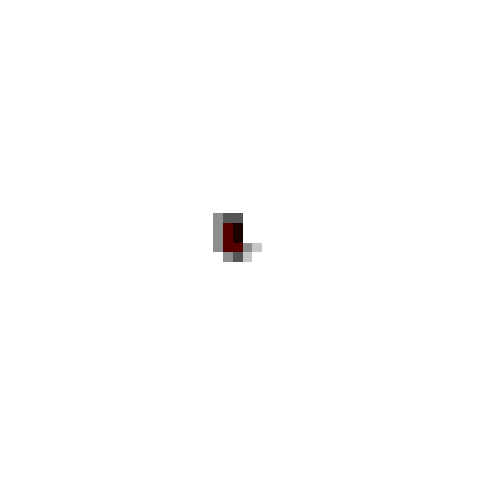
\includegraphics[height=2.5cm,width=2.5cm, frame]{fig/experimentos_base/images_parametros_padrao_area_artificial_moore_popnaohomogenea/epidemicmodel_t5.png}}}
\qquad
\subfloat[\textit{t} = 10]{{
\includegraphics[height=2.5cm,width=2.5cm, frame]{fig/experimentos_base/images_parametros_padrao_area_artificial_moore_popnaohomogenea/epidemicmodel_t10.png}}}
\qquad
\subfloat[\textit{t} = 15]{{
\includegraphics[height=2.5cm,width=2.5cm, frame]{fig/experimentos_base/images_parametros_padrao_area_artificial_moore_popnaohomogenea/epidemicmodel_t15.png}}}
\qquad
\subfloat[\textit{t} = 25]{{
\includegraphics[height=2.5cm,width=2.5cm, frame]{fig/experimentos_base/images_parametros_padrao_area_artificial_moore_popnaohomogenea/epidemicmodel_t25.png}}}
\qquad
\subfloat[\textit{t} = 35]{{
\includegraphics[height=2.5cm,width=2.5cm, frame]{fig/experimentos_base/images_parametros_padrao_area_artificial_moore_popnaohomogenea/epidemicmodel_t35.png}}}
\qquad
\subfloat[\textit{t} = 50]{{
\includegraphics[height=2.5cm,width=2.5cm, frame]{fig/experimentos_base/images_parametros_padrao_area_artificial_moore_popnaohomogenea/epidemicmodel_t50.png}}}
\qquad
\subfloat[\textit{t} = 60]{{
\includegraphics[height=2.5cm,width=2.5cm, frame]{fig/experimentos_base/images_parametros_padrao_area_artificial_moore_popnaohomogenea/epidemicmodel_t65.png}}}
\caption{Simulação com população variável ($e^j$) e vizinhança de Moore com conectividade por quadrante}
\label{figure:exp3moore}
\end{figure}

\subsubsection{Vacinação na população}

O modelo analisado neste Trabalho considera também a disponibilização de vacinas para o controle da epidemia. Desta forma, para a verificação do comportamento do modelo, é realizado um teste onde é simulado a criação de uma vacina, que não ocorre no início da epidemia, assim, o fator de vacinação começa a ser aplicado somente após $t = 15$. A Figura \ref{figure:vac1moore} apresenta o resultado de uma simulação utilizando a vizinhança de Moore e um fator de vacinação $\omega = 0.2$, neste é possível perceber que, logo após a aplicação da vacina, a quantidade de infectados começa a diminuir de forma muito rápida. 

% vac1
\begin{figure}[!ht]
\captionsetup[subfigure]{labelformat=empty}
\centering
\subfloat[\textit{t} = 1]{{\includegraphics[height=2.5cm,width=2.5cm, frame]{fig/experimentos_base/images_parametros_padrao_vacina_0-2/epidemicmodel_t1.png}}}
\qquad
\subfloat[\textit{t} = 5]{{\includegraphics[height=2.5cm,width=2.5cm, frame]{fig/experimentos_base/images_parametros_padrao_vacina_0-2/epidemicmodel_t5.png}}}
\qquad
\subfloat[\textit{t} = 10]{{
\includegraphics[height=2.5cm,width=2.5cm, frame]{fig/experimentos_base/images_parametros_padrao_vacina_0-2/epidemicmodel_t10.png}}}
\qquad
\subfloat[\textit{t} = 15]{{
\includegraphics[height=2.5cm,width=2.5cm, frame]{fig/experimentos_base/images_parametros_padrao_vacina_0-2/epidemicmodel_t15.png}}}
\qquad
\subfloat[\textit{t} = 18]{{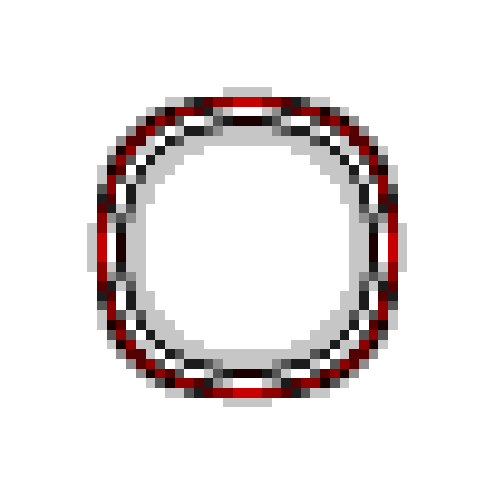
\includegraphics[height=2.5cm,width=2.5cm, frame]{fig/experimentos_base/images_parametros_padrao_vacina_0-2/epidemicmodel_t18.png}}}
\qquad
\subfloat[\textit{t} = 20]{{
\includegraphics[height=2.5cm,width=2.5cm, frame]{fig/experimentos_base/images_parametros_padrao_vacina_0-2/epidemicmodel_t20.png}}}
\qquad
\subfloat[\textit{t} = 21]{{\includegraphics[height=2.5cm,width=2.5cm, frame]{fig/experimentos_base/images_parametros_padrao_vacina_0-2/epidemicmodel_t21.png}}}
\qquad
\subfloat[\textit{t} = 23]{{\includegraphics[height=2.5cm,width=2.5cm, frame]{fig/experimentos_base/images_parametros_padrao_vacina_0-2/epidemicmodel_t23.png}}}
\caption{Simulação com população constante e vizinhança de Moore com vacinação igualmente distribuída}
\label{figure:vac1moore}
\end{figure}

% \newpage

Como os parâmetros utilizados para este testes são os mesmos empregados anteriormente, é possível realizar um comparativo para entender a eficácia do fator de vacinação. Perceba que na Figura \ref{figure:exp1moore} a epidemia continua a se espalhar até o final do espaço celular, o que indica que, mesmo havendo recuperação dos indivíduos infectados, o vírus se manteria entre a população, mas, ao considerar a vacinação, como apresentado na Figura \ref{figure:vac1moore} a epidemia não foi apenas parada, como a quantidade de infectados vai para zero, antes mesmo de atingir $t = 30$. É interessante notar que todo este comportamento ocorreu mesmo com um fator de vacinação $\omega = 0.2$.

\subsection{Aplicação do modelo}

Como forma de realizar a aplicação do modelo, foi realizado um processo de espacialização do mesmo. A área de aplicação do modelo representa o território brasileiro, como espaço celular, onde são consideradas condições espaciais para população (a população de cada estado), conectividade (fator definido pelo número de aeroportos por estado) e capacidade de vacinação (Proporcional ao desenvolvimento econômico estadual). O valor desses fatores são apresentados no intervalo $[0,1]$, sendo gerados com a normalização considerando os valores do estado de São Paulo. A Figura \ref{figure:CI} apresenta a forma e intensidade que cada uma dessas variáveis em seus respectivos estados. 

\begin{figure}[!ht]
 \begin{center}
  \includegraphics[width=1\linewidth]{fig/variaveis_espaciais.png}
 \end{center}
 \caption{Condições espaciais heterogêneas.}
\label{figure:CI}
\end{figure}

Para a verificação do comportamento, foram gerados 4 testes, sendo cada um desses especificados na Tabela \ref{tab:exp}. Em todos os casos foi adotado que o estado de São Paulo foi o ponto de início da epidemia, além de que o fator de recuperação ($\varepsilon$) usado, será igual a 0, a virulência ($v$) igual a $0.6$, uma movimentação (m) de $0.2$ e 200 instantes de tempo.

\begin{table}[ht]
 \caption{Experimentos realizados no modelo espacializado}
 \centering
 \begin{tabular}{c|c|c|c|c}
  Experimento & Vizinhança & População & Conectividade & Vacinação \\
  \hline
  \multirow{2}{*}{1} & Moore & \multirow{2}{*}{Homogênea} & \multirow{2}{*}{Homogênea} & \multirow{2}{*}{Não} \\
   & Neumman &  &  &  \\
  \hline
  \multirow{2}{*}{2} & \multirow{2}{*}{Moore} & Homogênea & \multirow{2}{*}{Homogênea} & \multirow{2}{*}{Não} \\
  &  & Heterogênea &  &  \\
  \hline
  \multirow{2}{*}{3} & \multirow{2}{*}{Moore} & \multirow{2}{*}{Homogênea} & Homogênea & \multirow{2}{*}{Não} \\
  &  &  & Heterogênea &  \\
  \hline
  \multirow{2}{*}{4} & \multirow{2}{*}{Moore} & \multirow{2}{*}{Homogênea} & \multirow{2}{*}{Homogênea} & Sim \\
  &  &  &  & Não \\
\end{tabular}
\label{tab:exp}
\end{table}

\newpage

A Figura \ref{fig:exp_espa} mostra os resultados dos experimentos realizados para o último tempo $t=199$, onde o experimento 1 é considerado como referência.

\begin{figure}[!ht]
\centering
\subfloat[Experimento 1]{\includegraphics[height=7cm,width=7cm, frame]{fig/exp1.png}}
\qquad
\subfloat[Experimento 2]{\includegraphics[height=7cm,width=7cm, frame]{fig/exp2.png}}

\subfloat[Experimento 3]{\includegraphics[height=7cm,width=7cm, frame]{fig/exp3.png}}
\qquad
\subfloat[Experimento 4]{\includegraphics[height=7cm,width=7cm, frame]{fig/exp4.png}}
\caption{Resultados para a espacialização do modelo.}
\label{fig:exp_espa}
\end{figure}

A partir do experimento 2 pode-se observar um aumento no número de infectados para o nordeste do Brasil (em relação ao experimento controle), porque a população nessa região é maior do que na região centro-oeste. No experimento 3, o avanço do vírus é muito maior do que no experimento 2, em termos de número de infectados, isto porque a região centro-oeste apresenta boa conectividade, portanto, a diferença com a região nordeste não é muito acentuada, sendo benéfico para a propagação do vírus, já que a propagação é muito maior que no experimento referência. Finalmente, o experimento 4 mostra os resultados da presença de um plano de vacinação, onde os estados com maior investimento mostram o menor número de infectados, sendo esta a única maneira de impedir o avanço do vírus.

\newpage


Cabe notar também que, no mapa de vacinação apresentado na Figura \ref{figure:CI}, o Sul, Sudeste e Nordeste de Brasil apresentam programas de vacinação e o Norte e Centro-Oeste não. Ao considerar tal mapa, na Figura \ref{fig:exp_espa} (d), pode-se observar que os estados com maior fator de vacinação são os que apresentaram o menor numero de infectados. Por exemplo, devido ao programa de vacinação presente em São Paulo ser um fator igual a 0.2, o avanço do vírus é muito menor do que em um cenário sem presença de vacina, o que também ocorre em estados com fator de vacinação igual ou próximo, como Minas Gerais, Santa Catarina, Rio Grande do Sul e Rio de Janeiro. Porém, ao considerar estados como Paraná, que possuem um fator de vacinação igual a 0.1, o número de infectados é muito maior, podendo neste caso, ser até mesmo considerado o maior na região sul do Brasil. Para os estados que não têm vacinação, no tempo 199 o vírus atinge sua capacidade máxima de infecção como pode ser visto no Mato Grosso.

\section{Conclusões}


O presente trabalho teve como principal objetivo implementar o modelo de AC, proposto por White 2007 \cite{White2007}, este que através de um conjunto de regras simples, e diferentes tipos de população busca modelar cenários de epidemias de diferentes doenças. Ao realizar a implementação do modelo e a geração dos casos de teste seguindo as definições apresentadas no artigo do modelo, pode-se afirmar que os resultados obtidos neste trabalho apresentam comportamento semelhante ao do artigo base. Além disso, através da aplicação do modelo analisado em um cenário que considera informações reais de estados brasileiros, foi possível perceber um comportamento parecido com os realizados nos testes e ainda, podendo ser vinculado também a epidemias reais, mesmo que a epidemia gerada para estes testes considere parâmetros sintéticos para a representação das capacidades da doença simulada.

Com base nos resultados, pode-se observar que variações na conectividade geram um maior impacto do vírus, ou seja, para esse cenário, é apresentado um número maior de pessoas infectadas, diferentemente da população não homogênea. Essa diferença provavelmente se deve ao fato de que variações na população causam um número maior de infecções para uma determinada célula, enquanto uma maior conectividade implica uma maior transferência de indivíduos entre as células, onde, em um determinado momento, um indivíduo infectado ingressa em outra célula e o vírus com ele, isto acontece principalmente em células altamente conectadas, conhecidas como \textit{hubs}.

Com isto, é possível afirmar que o modelo implementado e analisado neste trabalho, mesmo não realizando considerações complexas do espalhamento de uma epidemia, consegue realizar a modelagem de cenários próximos aos de epidemias reais, da mesma forma como proposta, sendo necessário definições coerentes dos parâmetros no momento da modelagem.

\newpage
\bibliographystyle{acm}
\bibliography{bibfile}

\end{document}
